%%%%%%%%%%%%%%%%%%%%%%%%%%%%%%%%%%%%%%%%%%%%%%%%%%
%%%%%%%%%%%%%%%%%%%%%%%%%%%%%%%%%%%%%%%%%%%%%%%%%%
%%%%%%%%%%%%%%%%%%%%%%%%%%%%%%%%%%%%%%%%%%%%%%%%%%
% PREAMBLE:

\documentclass[12pt,a2paper,landscape]{article}

%%%%%%%%%%%%%%%%%%%%%%%%%%%%%%%%%%%%%%%%%%%%%%%%%%

\usepackage[noheadfoot,margin=10mm]{geometry}
% width=554mm,height=400mm
\usepackage[utf8]{inputenc}
\usepackage[english]{babel}
\usepackage{graphicx,multicol,color} 
%\usepackage{everyshi,eso-pic,calc,ifthen,wallpaper} 
\usepackage{tikz}
\usepackage{amsmath,amsfonts,amssymb,amsthm}
\usetikzlibrary{automata,arrows,positioning,calc}
\usepackage{mathtools}
\usepackage{caption}
\usepackage{anyfontsize}

%%%%%%%%%%%%%%%%%%%%%%%%%%%%%%%%%%%%%%%%%%%%%%%%%%

\pagestyle{empty}
\definecolor{cola}{rgb}{.99,.93,0}
\definecolor{colb}{rgb}{.8,0,.7}
\definecolor{colc}{rgb}{1,.9,.9}
\DeclarePairedDelimiter\abs{\lvert}{\rvert}

%% boxes to put stuff in ......
%%
%%   (1) transparent boxes --- the background shows through
%%			   #1 = width as fraction of what's available
%%                         #2 = contents (text, formula, picture)
%%                               ... tho pictures are always opaque
%% ---- box for headers --- width = fraction of textwidth 

\newcommand\BoX[2]{\begin{minipage}{#1\textwidth}#2\end{minipage}}
%% ---- box centred in a column --- width = fraction of columnwidth
\newcommand\BOX[2]{\begin{center}
   \begin{minipage}{#1\columnwidth}#2\end{minipage}\end{center}\vfill}
%%
%%   (2) opaque boxes with coloured background and outline frame
%%                         #1 = width as fraction of what's available
%%                         #2 = contents (text, formula, picture)
%%                         #3 = background colour
%%                         #4 = frame colour
\setlength\fboxrule{2pt} %% = width of frame lines round boxes
\setlength\fboxsep{5pt}  %% = spacing round box contents
%% ---- box for headers --- width = fraction of textwidth 
\newcommand\cBoX[4]{\fcolorbox{#4}{#3}{%
	\begin{minipage}{#1\textwidth}#2\end{minipage}}}
%% ---- box centred in a column --- width = fraction of columnwidth
\newcommand\cBOX[4]{\begin{center}\fcolorbox{#4}{#3}{%
 \begin{minipage}{#1\columnwidth}#2\end{minipage}}\end{center}\vfill}


%% for e.g. picture and text side-by-side in a column
%%   n.b. this command must be inside a \BOX or a \cBOX
\newcommand\sidebyside[2]{\BoX{.485}{#1}\BoX{.485}{#2}}

\def\bibsection{\section*{References}}        % Position reference section correctly

\renewcommand\familydefault{\sfdefault}

\newtheorem{definition}{Definition}[section]
\newtheorem{exmp}{Example}[section]
\newtheorem*{theorem*}{Theorem}
\DeclareMathOperator{\sech}{sech}		% Defining sech so it doesn't italicise it 
\DeclareMathOperator{\Int}{Int}		% Defining 'integer part of' so it doesn't italicise it 

\setlength\columnsep{10mm}  %%%% column separation

%%%%%%%%%%%%%%%%%%%%%%%%%%%%%%%%%%%%%%%%%%%%%%%%%%
%%%%%%%%%%%%%%%%%%%%%%%%%%%%%%%%%%%%%%%%%%%%%%%%%%
%%%%%%%%%%%%%%%%%%%%%%%%%%%%%%%%%%%%%%%%%%%%%%%%%%
% DOCUMENT

\begin{document}
%\tikz[remember picture,overlay] \node[inner sep=0pt] at (current page.center)
%{ 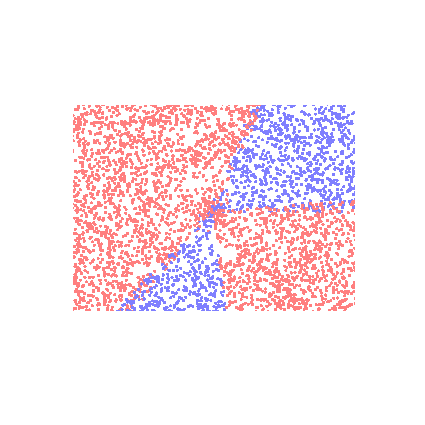
\includegraphics[width=\paperwidth,height=\paperheight]{spiral3.pdf}};

\begin{tikzpicture}[remember picture, overlay]
  \node [anchor=north west, inner sep=1cm]  at (current page.north west)
     {
\includegraphics[height=3cm]{university}};
\end{tikzpicture}
\hfill
\cBoX{0.75}{\centering
\vspace{1ex}
{\fontsize{1.8cm}{2cm}\selectfont{\textsc{Solitons in a Bose-Einstein Condensate \\}}}
\huge
\textsc{L P Flower\\
Project Tutor: Dr. Rahul Sawant}
\vspace{1ex}
}{white}{white}
\hfill
%\cBoX{.3}{\color{black}
%\centering
%\huge
%\textsc{L P Flower\\
%Project Tutor: \\
%Dr. Rahul Sawant}
%}{white}{white}
\vspace{0.5in} 

%%%%%%%%%%%%%%%%%%%%%%%%%%%%%%%%%%%%%%%%%%%%%%%%%%
%%%%%%%%%%%%%%%%%%%%%%%%%%%%%%%%%%%%%%%%%%%%%%%%%%
%%%  now the body material in 3 columns of stacked boxes
%%      ... use \BOX and/or \cBOX here

\begin{multicols*}{3}
\setlength\fboxrule{1pt} 

%%%   to get more in, try say 4 columns with smaller-sized type
%%%  BUT -- for easy reading 
%%%               use no more than about 66 characters per line
%%%%   .... and choose a size of type that 
%%%%              looks OK expanded from A4 to A2
% \tiny
\small


%%%%%%%%%%%%%%%%%%%%%%%%%%%%%%%%%%%%%%%%%%%%%%%%%%

\fboxsep=5.5pt

\cBOX{0.97}{\section*{Introduction}
{
\fontsize{16pt}{20pt}\selectfont
The atoms in a Bose-Einstein condensate are all described by the same wavefunction, since they are in the same quantum state, which includes each atom's interaction with the other atoms in the condensate. Introducing an pseudopotential term $g \abs{\psi}^2$ which characterises the interactions between the particles into the dimensionless Schr\"{o}dinger equation yields the Gross-Pitaevskii equation \cite{}
\begin{equation}
i \frac{\partial \psi}{\partial t} = -\frac{\partial^2 \psi}{\partial x^2} + (V + g \abs{\psi}^2) \psi,
\end{equation}
where $\psi$ is the atomic wavefunction, $t$ and $x$ are the rescaled time and length variables, $V$ is the external potential (if present) and $g$ is the interaction parameter. 

It is usual to define $\zeta$ as a parameter to characterise width, with units of inverse length. The normalised wavefunction is then
\begin{equation} 
\psi(x) = \sqrt{\frac{\zeta}{2}} \sech{(\zeta x)} e^{i v x + \phi},
\end{equation}
where $v$ is the velocity of the soliton and $\phi$ is a phase factor. 
Substituting the $v=0$ case into the time-independent Schrodinger equation and setting E to be $\zeta^2$, we find $g=4\zeta$. 

\section*{Propagating a Soliton}

The Gross-Pitaevskii equation was solved numerically using the split-step Fourier method \cite{}. 

\begin{center}
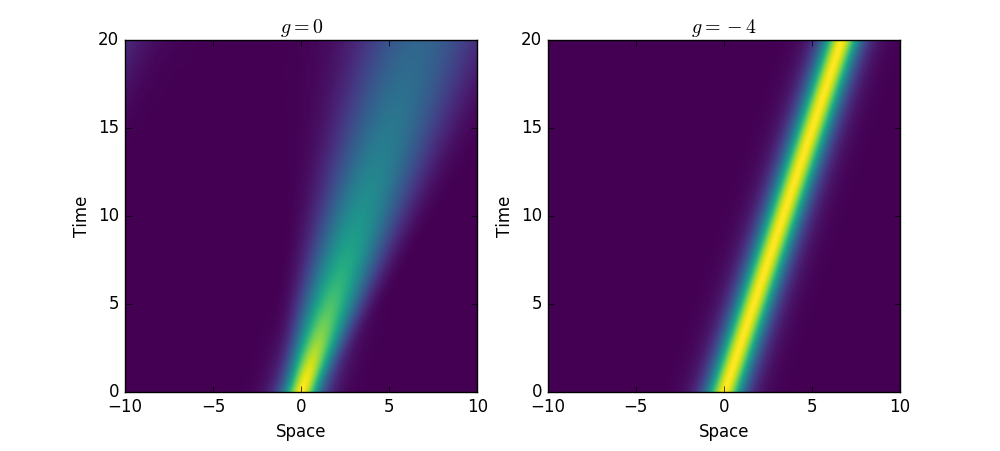
\includegraphics[scale=0.5]{milestonepic.png}
\captionof{figure}{$n=50$, $p=0.6$}
\end{center}


%\subsection*{Exclusion Process}
%The exclusion process is slightly different from the previous processes. Here two coordinates of $\eta_{t}$
%change at a time. Particles move on $I$ in the following way.
%\begin{itemize}
%	\item[(a)] At most one particle occupies a site $x \in I$;
%	\item[(b)] A particle at $x$ waits for a time $\sim Exp(1)$ and then chooses a site $y \in I$ with probability
%	$p(x,y)$ given by the transition probabilities for a discrete time Markov chain on $I$;
%	\item[(c)] If $y$ is vacant at that time, the particle moves to $y$, otherwise it remains at $x$.
%\end{itemize}
%Once again $\eta(x)=1$ corresponds to occupation and $\eta(x)=0$ corresponds to vacancy.
}
}{white}{white}

%%%%%%%%%%%%%%%%%%%%%%%%%%%%%%%%%%%%%%%%%%%%%%%%%%

\cBOX{0.97}{\section*{Richardson Growth Model}
This model is constructed by attaching independent Poisson Processes $T_{n}^{(x,y)}$
of rate $1$ for each of its $y$ neighbours, where
$n$ denotes the $n$\textsuperscript{th} arrival, to $x$. If at time $T_{n}^{(x,y)}$ we have $x \in \xi_{t}$ 
and $y \notin \xi_{t}$ we add $y$ to $\xi_{t}$.
\vspace{1ex}

Take $d=1$, $A=\{0\}$ and let $t(n)=\inf\{t : n \in \xi_{t}^{\{0\}}\}$, that is, $t(n)$ is the time taken 
for $n \in \mathbb{Z}$ to become occupied. Suppose $n>0$, then the only way to occupy $n$ 
is to first occupy $1,2,\cdots,n-1$ successively. The interarrival times
are exponentially distributed with parameter 1, and the memoryless property of the exponential
distribution gives us that each successive occupation is independent. Hence by an application 
of the strong law of large numbers we get that $t(n)/n \rightarrow 1$ almost surely. So we can 
see that $\xi_{t}$ grows somewhat linearly when $d=1$.

Now for $d \geq 1$ define a thickened version of our set of occupied sites, $\xi_{t}^{\{0\}}$, as follows
\begin{equation*}
\bar{\xi}_{t}^{\{0\}} := \Big\{ x + y : x \in \xi_{t}^{\{0\}}, y \in \Big[-\frac{1}{2},\frac{1}{2}\Big]^{d} \Big\}
\end{equation*}
This gives rise to the following result for the limiting shape.
}{white}{white}

%%%%%%%%%%%%%%%%%%%%%%%%%%%%%%%%%%%%%%%%%%%%%%%%%%

\columnbreak
\cBOX{0.97}{\subsection*{}
\begin{theorem*}
Let $\epsilon>0$ be given, then $\exists$ a convex set $A$ s.t.
\begin{equation*}
P\Big[(1-\epsilon)tA \subset \bar{\xi}_{t}^{\{0\}} \subset (1+ \epsilon)tA\Big] \rightarrow 1 
\mbox{ as } t \rightarrow \infty
\end{equation*}
\end{theorem*}

If $\xi_{t(x)+u}^{(x,t(x))}$ is the set of sites that can be reached
after time $u$ from $x$ at time $t(x)$, we define 
$$t(x,y) = \inf\{ u : y \in \xi_{t(x)+u}^{(x,t(x))}\}$$ 
We have that $t(x,y)$ is independent of $t(x)$ by properties 
of the Poisson process and $t(x,y)$ has the same distribution has $t(y-x)$ by translational 
symmetry of the lattice. 
\vspace{1ex}

Taking $n \in \mathbb{Z}$ one can use the subadditive ergodic theorem to obtain that
$t(0,nx)/n \rightarrow$ some limit $\mu(x)$ as $n \rightarrow \infty$, so in particular we have that
$\xi_{t}^{\{0\}}$ grows linearly in each direction. By setting $t(x)= \inf\{t: x \in \bar{\xi}_{t}^{\{0\}}\}$
we extend $t(x)$ to all $x \in \mathbb{R}^{d}$. It is possible to show that
\begin{equation*}
\frac{t(nx)}{n} \rightarrow \mu(x) \mbox{ a.s. } \forall x \in \mathbb{R}^{d}
\end{equation*}
It turns out that $\mu$, given by $\inf_{m\geq 1}\frac{E(t(mx))}{m}$, defines a norm on 
$\mathbb{R}^{d}$. The convex set $A$ in the theorem is given by the unit ball in that norm.
In particular for $\mathbb{Z}^{2}$ we see that $\bar\xi_{t}^{\{0\}}/t$ is, in the
sense of the norm $\mu$, roughly circular. However it is very difficult to compute $\mu$ from
this expression, so it does not really tell us much about how our process is growing.
\vspace{1ex}
 
To get a better feel for the norm and the limiting shape of the growth model we will pass to a 
discrete version of the process on $\mathbb{Z}^{2}$.
}{white}{white}

%%%%%%%%%%%%%%%%%%%%%%%%%%%%%%%%%%%%%%%%%%%%%%%%%%

\cBOX{0.97}{
%\subsection*{Understanding the limiting shape}
%The discrete version of the Richardson growth model follows the same rules, but if a site is vacant at
%time $n$, and at least one of its neighbours is occupied, it becomes occupied with probability $p$.
%Decisions at different times and different sites are made independently. Just
%as for the continuous case, we have an asymptotic shape result.
%\vspace{1ex}
%
%For any $p \in (0,1)$ there exists a norm $\mu_{p}(x)$ on $\mathbb{R}^{2}$, and for any $\epsilon > 0$,
%$$P\Big[\{\mu_{p} \leq 1-\epsilon \} \subset \frac{\bar{\xi}_{n}^{\{0\}}}{n} \subset
%\{\mu_{p} \leq 1+\epsilon \}\Big] \rightarrow 1 \mbox{ as } n \rightarrow \infty$$

\subsection*{Flat edges}
We identify an embedded discrete contact process given by $\zeta_{n}(x)= \eta_{n}(x,n-x)$, where
$x \in \mathbb{Z}$. It is known for the contact process that $\exists \mbox{\phantom{Z}} p_{0}<1$ such that 
$p>p_{0} \Rightarrow P(\zeta_{n} \not\equiv 0 \mbox{ for all } n) >0$, so the inclusion 
$\{x \in \mathbb{Z}^{2}: \eta_{n}(x) =1\} \supset \{(y,n-y): \zeta_{n}(y)=1\}$ gives us that
for  $P(\zeta_{n} \not\equiv 0 \mbox{ for all } n) >0$
\begin{equation*}
B_{p}:=\{x:\mu_{p}(x) \leq{1}\} \cap \{x: x_{1}+x_{2}=1\} \neq \phi
\end{equation*}
Symmetry arguments yield that $(1/2,1/2) \in B_{p}$, and if we define
$p_{cr} =  \inf\{p: P(\zeta_{n} \not\equiv 0 \mbox{ for all } n) >0\}$, then the result reads that 
for $p>p_{cr}, (1/2, 1/2) \in B_{p} \mbox{ and } \mu_{p}(1/2, 1/2)=1$.
\vspace{1ex}

It can be shown that for $p>p_{cr}$, we have $\partial B_{p} \cap \{x: x_{1}+x_{2}=1\}$
is an interval of length at least $2\sqrt{2}\mbox{\phantom{.}}[p-p_{cr}]$. This means that in the limit of our rescaled
set of occupied points, the boundary has edges that look flat.
\vspace{1ex}

In fact simulations of the discrete Richardson growth model, you see that for $p$ close 
to $1$, the limiting shape is close to a diamond, but as $p$ varies from $1$ to $0$, 
the limiting shape becomes more and more circular.
}{white}{white}

%%%%%%%%%%%%%%%%%%%%%%%%%%%%%%%%%%%%%%%%%%%%%%%%%%

\cBOX{0.97}{\subsection*{Discrete simulations in Python}
Colouring only the boundary, we can see the shape of the rescaled set of occupied points.
\sidebyside{
\hspace{7ex}
\begin{center}
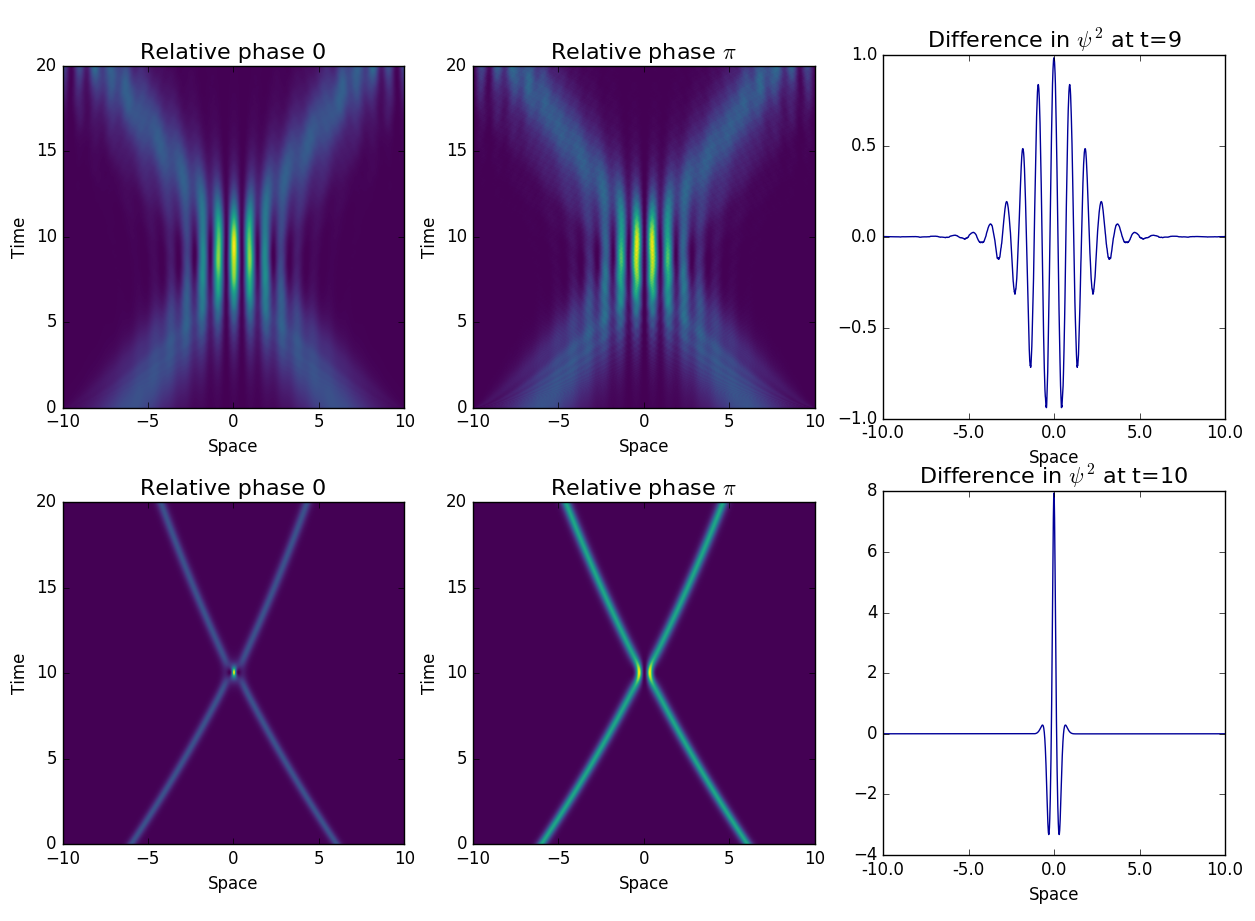
\includegraphics[scale=0.28]{extensionpic.png}
\captionof{figure}{$n=50$, $p=0.6$}
\end{center}
}
{
\hspace{6ex}
%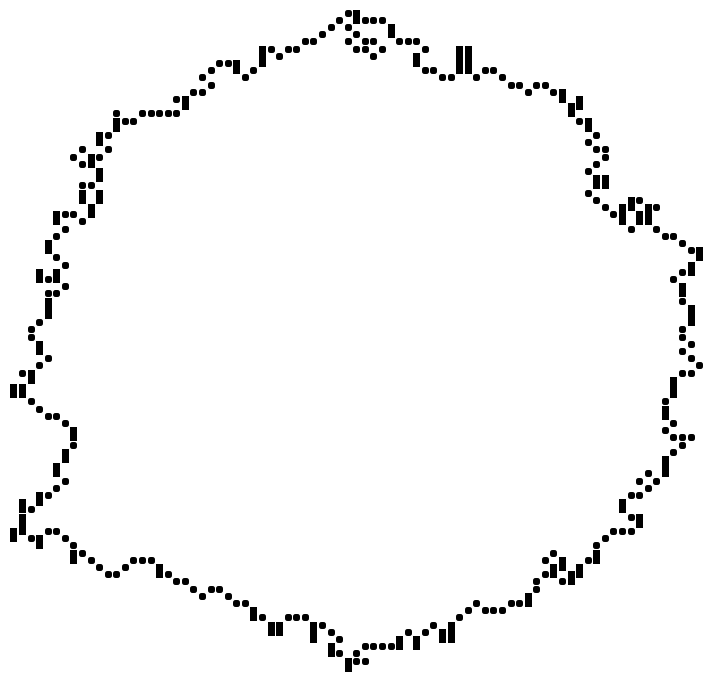
\includegraphics[scale=0.30]{pic1.png}
%\captionof{figure}{$n=200$, $p=0.1$}
}
}{white}{white}

%%%%%%%%%%%%%%%%%%%%%%%%%%%%%%%%%%%%%%%%%%%%%%%%%%

\columnbreak
\cBOX{0.97}{
\subsection*{The two-type Richardson growth model}
For two different types of particles, type I and type II, on $\mathbb{Z}^{d}$ we define the two-type
Richardson growth model in a similar manner. Vacant sites are occupied by a particle of type I or 
type II at a rate given by the number of neighbours of a given type multiplied by parameters
$\lambda_{1}, \lambda_{2}$ respectively. Once a particle occupies a site, it occupies it for all
future times. Starting from a single occupied site for each type, it is not clear whether the sets of 
occupied sites for each types can both grow to be infinite. For example it can happen that one 
set completely surrounds the other and prevents further growth.
\vspace{1ex}

It is conjectured that for $d \geq 2$, starting from single sites, the probability that the sets of occupied
sites can both grow to infinite size is positive if and only if $\lambda_{1}=\lambda_{2}$. 
\vspace{1ex}

It is known that for all but at most countably many values of $\lambda := \lambda_{2}/\lambda_{1}$,
the probability that both sets of occupied sites can grow to be infinite is $0$.

%\subsection*{Central limit theorem}
%So far we have seen that we have a law of large numbers for $t(nx)$, but we have said nothing about the
%its fluctuations. It can be shown that they are bounded by $\sqrt{n}$, but several simulations have indicated 
%that its fluctuations are more likely to be of order $n^{1/3}$.
}{white}{white}

%%%%%%%%%%%%%%%%%%%%%%%%%%%%%%%%%%%%%%%%%%%%%%%%%%

\cBOX{0.97}{\section*{Repeated Collisions}

%\sidebyside{
\begin{center}
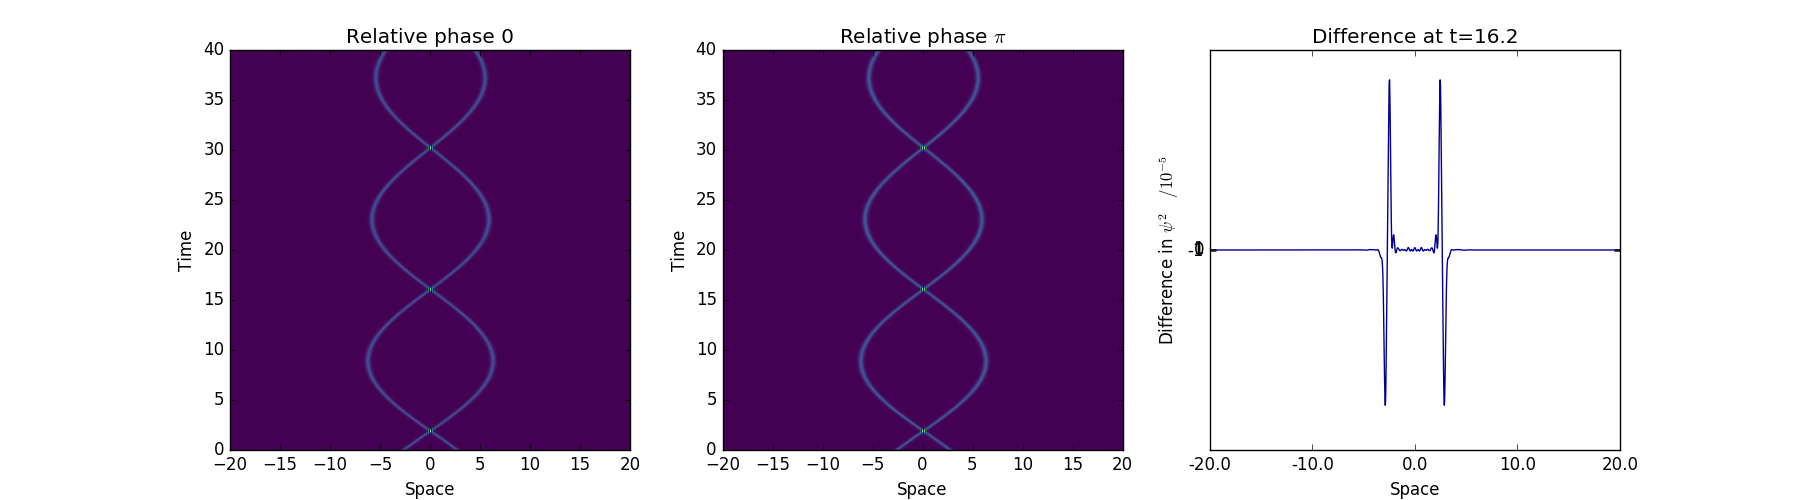
\includegraphics[width=\columnwidth]{difference.png}
\captionof{figure}{$n=50$, $p=0.6$}
\end{center}
%}
%{\vspace{1ex}Supposing this graph represents the process for $d=1$, then
%the opinion of individual $0$ at time $t$ is the same as that of individual $-2$ 
%at time $0$, and if we set $A=\{-2\}$ we get that $\xi_{t}^{\{-2\}}=\{-3,-2,-1,0\}$.

}{white}{white}

%%%%%%%%%%%%%%%%%%%%%%%%%%%%%%%%%%%%%%%%%%%%%%%%%%

%\cBOX{0.97}{\section*{Contact Process}
%This process can also be constructed graphically. To $x \in I$ attach independent Poisson processes
%$\{T_{n}^{(x,y)}, n \geq 1\}$ of rate $\lambda$ for each neighbour $y$ and $\{U_{n}^{x}, n \geq 1\}$ of
%rate $1$. For the times $T_{n}^{(x,y)}$ draw an arrow from $x$ to $y$ and write at $\delta$ at times
%$U_{n}^{x}$. Paths and $\xi_{t}^{A}$ are defined as they were in the Voter model.

%If we take $I=\mathbb{Z}^{d}$ it is not clear if the process survives. If we take $\lambda \leq 1/2d$
%the maximal rate of infection for any individual is less than its healing rate, and the process will
%die out almost surely.

%In the situation of the finite graph approximate results are known for the expected lifetime of 
%the infection. 
%}{white}{black}

%%%%%%%%%%%%%%%%%%%%%%%%%%%%%%%%%%%%%%%%%%%%%%%%%%

\vspace{-2cm}
\cBOX{0.97}{
\subsection*{Threshold voter model}
The voter model we defined above is in fact a particular case of the linear voter model.
There are nonlinear models such as the threshold voter model. If we intersect $\mathbb{Z}^{d}$
with a compact, convex and symmetric set $X \subset \mathbb{R}^{d}$ we obtain a neighbourhood
$\mathcal{N}=X \cap \mathbb{Z}^{d}$ of $0$. For a positive integer $T$, the threshold model
corresponding to $\mathcal{N}$ and $T$ has rate function
\begin{equation*}
c(x, \eta)=
\begin{cases}
1 & \mbox{ if } \#\{y \in x + \mathcal{N}: \eta(y) \neq \eta(x)\}\geq T\\
0 & \mbox{ otherwise.}
\end{cases}
\end{equation*}
}{white}{white}

%%%%%%%%%%%%%%%%%%%%%%%%%%%%%%%%%%%%%%%%%%%%%%%%%%

\vspace{-2cm}
\cBOX{0.97}{\section*{Final Remarks}
Each of the models presented here can be studied in greater generality, for
various index sets $I$. There are many results for processes taking $I=V$ for 
some vertex set $V$ of a connected undirected graph $G=(V,E)$, whose
vertices have bounded degrees.
}{white}{white}

%%%%%%%%%%%%%%%%%%%%%%%%%%%%%%%%%%%%%%%%%%%%%%%%%%

\vspace{-1.9cm}
\cBOX{0.97}{

\begin{thebibliography}{}

\bibitem{KdV} D. J. Korteweg and G. de Vries (1895), "On the Change of Form...", \textit{Philosophical Magazine} \textbf{39}(240) pp. 422-443.

\bibitem{Segur} H. Segur (1973), "The Korteweg de Vries equation and water waves, part 1", \textit{Journal of Fluid Mechanics} \textbf{59} pp. 721-736.

\bibitem{Gardner} C. S. Gardner et al. (1967), "Method for Solving the Korteweg de Vries Equation", \textit{Physical Review Letters} \textbf{19}(19) pp. 1095-1097.

\bibitem{UGlab} Alessandro Bettini et al. (1983), "Solitons in Undergraduate Laboratory", \textit{American Journal of Physics} \textbf{51}(11).

\bibitem{Hughes} Ifan G. Hughes and Thomas P. A. Hase (2010), \textit{Measurements and their Uncertainties}.

\end{thebibliography} 

}{white}{white}
\end{multicols*}
\end{document}

%%%%%%%%%%%%%%%%%%%%%%%%%%%%%%%%%%%%%%%%%%%%%%%%%%
%%%%%%%%%%%%%%%%%%%%%%%%%%%%%%%%%%%%%%%%%%%%%%%%%%
